

\documentclass[11pt,compress,t,notes=noshow]{beamer}

\usepackage[]{color}


\def\maxwidth{ %
  \ifdim\Gin@nat@width>\linewidth
    \linewidth
  \else
    \Gin@nat@width
  \fi
}
\makeatother

\definecolor{fgcolor}{rgb}{0.345, 0.345, 0.345}
\newcommand{\hlnum}[1]{\textcolor[rgb]{0.686,0.059,0.569}{#1}}%
\newcommand{\hlstr}[1]{\textcolor[rgb]{0.192,0.494,0.8}{#1}}%
\newcommand{\hlcom}[1]{\textcolor[rgb]{0.678,0.584,0.686}{\textit{#1}}}%
\newcommand{\hlopt}[1]{\textcolor[rgb]{0,0,0}{#1}}%
\newcommand{\hlstd}[1]{\textcolor[rgb]{0.345,0.345,0.345}{#1}}%
\newcommand{\hlkwa}[1]{\textcolor[rgb]{0.161,0.373,0.58}{\textbf{#1}}}%
\newcommand{\hlkwb}[1]{\textcolor[rgb]{0.69,0.353,0.396}{#1}}%
\newcommand{\hlkwc}[1]{\textcolor[rgb]{0.333,0.667,0.333}{#1}}%
\newcommand{\hlkwd}[1]{\textcolor[rgb]{0.737,0.353,0.396}{\textbf{#1}}}%
\let\hlipl\hlkwb

\usepackage{framed}
\newenvironment{kframe}{%
 \def\at@end@of@kframe{}%
 \ifinner\ifhmode%
  \def\at@end@of@kframe{\end{minipage}}%
  \begin{minipage}{\columnwidth}%
 \fi\fi%
 \def\FrameCommand##1{\hskip\@totalleftmargin \hskip-\fboxsep
 \colorbox{shadecolor}{##1}\hskip-\fboxsep
     \hskip-\linewidth \hskip-\@totalleftmargin \hskip\columnwidth}%
 \MakeFramed {\advance\hsize-\width
   \@totalleftmargin\z@ \linewidth\hsize
   \@setminipage}}%
 {\par\unskip\endMakeFramed%
 \at@end@of@kframe}
\makeatother

\definecolor{shadecolor}{rgb}{.97, .97, .97}
\definecolor{messagecolor}{rgb}{0, 0, 0}
\definecolor{warningcolor}{rgb}{1, 0, 1}
\definecolor{errorcolor}{rgb}{1, 0, 0}
\definecolor{code}{rgb}{0.97, 0.96, 1.0}
\newenvironment{knitrout}{}{} % an empty environment to be redefined in TeX

\usepackage{alltt}
\usepackage[utf8]{inputenc}


\usepackage[english]{babel}
\usepackage{dsfont}
\newcommand\bmmax{2}
\usepackage{verbatim}
\usepackage{amsmath}
\usepackage{amsfonts}
\usepackage{mathtools}
\usepackage{csquotes}
\usepackage{cmbright}
\usepackage{multirow}
\usepackage{longtable}
\usepackage{enumerate}
\usepackage[absolute,overlay]{textpos}
\usepackage{psfrag}
\usepackage{algorithm}
\usepackage{algorithmicx}
\usepackage{algpseudocode}
\usepackage{eqnarray}
\usepackage{multimedia}
\usepackage{media9}
\usepackage{bytefield}
\usepackage{animate}
\usepackage{tikz}
\usepackage{setspace}
\usepackage{wrapfig}

\usetikzlibrary{shapes,matrix,positioning,chains,arrows,shadows,decorations.pathmorphing,fit,backgrounds}
\usepackage{adjustbox}
\usepackage{colortbl}
\usepackage{tabularx} % for tables (incl. \hline)
\usepackage{arydshln} % Load after array, longtable, colortab and/or colortbl , otherwise problems with \hline in tabular env
\usepackage{etex} %increase registers for \dimenS to more than 256, otherwise we get "No room for a new \dimen"
\usepackage{graphicx}
\usepackage{placeins}
\usepackage{booktabs} %used in epr lectures
\usepackage{bm} % bold greek letters
\usepackage{bbm}
\usepackage{hyperref} % url citing
\usepackage{blkarray} % block arrays
\usepackage{listings} % block of code
\usepackage{xcolor} %colored math symbols
\usepackage{pgffor}
\usepackage{verbatimbox}
\usepackage{tcolorbox}
%\usepackage[export]{adjustbox}
\usepackage{siunitx}
\def\signed #1{{\leavevmode\unskip\nobreak\hfil\penalty50\hskip1em
  \hbox{}\nobreak\hfill #1%
  \parfillskip=0pt \finalhyphendemerits=0 \endgraf}}

%some colors
\definecolor{checkgreen}{HTML}{18A126}
\definecolor{errorred}{HTML}{FF0000}
\definecolor{blockbg}{HTML}{F7F7F7}
\definecolor{gray}{HTML}{A0A0A0}

% basic latex stuff
\newcommand{\col}{\par\colorbox{code}{\parbox{\textwidth}{\theverbbox}}\par}
\newcommand{\eg}{e.\,g.\xspace} %for example
\newcommand{\ie}{i.\,e.\xspace} %that is to say...
\newcommand{\pkg}[1]{{\fontseries{b}\selectfont #1}} %fontstyle for R packages
\newcommand{\lz}{\vspace{0.5cm}} %vertical space
\newcommand{\oneliner}[1] % Oneliner for important statements
{\begin{block}{}\begin{center}\begin{Large}#1\end{Large}\end{center}\end{block}}
\def\SpAr{\quad \Rightarrow \quad}

%new environments

\newenvironment{vbframe}  %frame with breaks and verbatim
{
 \begin{frame}[containsverbatim,allowframebreaks]
}
{
\end{frame}
}

\newenvironment{vframe}  %frame with verbatim without breaks (to avoid numbering one slided frames)
{
 \begin{frame}[containsverbatim]
}
{
\end{frame}
}

\newenvironment{blocki}[1]   % itemize block
{
 \begin{block}{#1}\begin{itemize}
}
{
\end{itemize}\end{block}
}

\newenvironment{fragileframe}[2]{  %fragile frame with framebreaks
\begin{frame}[allowframebreaks, fragile, environment = fragileframe]
\frametitle{#1}
#2}
{\end{frame}}

\newsavebox\mybox
\newenvironment{aquote}[1]
  {\savebox\mybox{#1}\begin{quote}\openautoquote\hspace*{-.7ex}}
  {\unskip\closeautoquote\vspace*{1mm}\signed{\usebox\mybox}\end{quote}}
  
\tikzset{
  %Define standard arrow tip
  >=stealth',
  %Define style for boxes
  punkt/.style={
    rectangle,
    rounded corners,
    draw=black, very thick,
    text width=6.5em,
    minimum height=2em,
    text centered},
  % Define arrow style
  pil/.style={
    ->,
    thick,
    shorten <=2pt,
    shorten >=2pt,}
}
\usepackage{subfig}


\newcommand{\myframe}[2]{  %short for frame with framebreaks
\begin{frame}[allowframebreaks]
\frametitle{#1}
#2
\end{frame}}

\newcommand{\remark}[1]{
  \textbf{Remark:} #1
}

\usepackage{../../style/lmu-lecture}

\let\code=\texttt
\let\proglang=\textsf

\setkeys{Gin}{width=0.9\textwidth}

\usetikzlibrary{shapes,arrows,automata,positioning,calc}

% Define block styles
\tikzstyle{decision} = [diamond, draw, text width=6em, text badly centered, node distance=4cm, inner sep=0pt]
\tikzstyle{decision2} = [diamond, draw, fill=customgreen!35, text width=6em, text badly centered, node distance=4cm, inner sep=0pt]

\tikzstyle{block} = [rectangle, draw, text width=14em, text centered, rounded corners, node distance=3cm, minimum height=4em]
\tikzstyle{line} = [draw, -latex']
\tikzstyle{cloud} = [draw, ellipse, node distance=3cm, minimum height=2em]

\title{Introduction to Deep Learning}
\author{Bernd Bischl}
\institute{Department of Statistics -- LMU Munich}
\date{WS 2021/2022}

\setbeamertemplate{frametitle}{\expandafter\uppercase\expandafter\insertframetitle}

\IfFileExists{upquote.sty}{\usepackage{upquote}}{}
\input{../../latex-math/basic-math}
\input{../../latex-math/basic-ml}

\begin{document}

\lecturechapter{0}{Introduction to Machine Learning}
\lecture{Deeplearning}

\begin{frame}{Data Science and Machine Learning}

\begin{columns}
  \column{.3\textwidth}
    \begin{figure}
      \includegraphics[width=\textwidth]{plots/gears.png}
    \end{figure}
  \column{0.6\textwidth}
  \begingroup
  \centering
    \fontsize{20pt}{22pt}\selectfont
    \vspace{1cm}
    \\
 % Machine Learning is a method of teaching computers to make predictions based on some data.
 %Machine learning is the study of algorithms that can automatically learn from and make predictions on data.
  Machine learning is a branch of computer science and applied statistics covering algorithms that improves their performance at a given task based on sample data or experience.
  \endgroup
\end{columns}

\end{frame}

\begin{frame}{Data Science and Machine Learning}

\scriptsize

\begin{center}
\includegraphics[width=0.95\textwidth]{plots/learning.pdf} 
\end{center}

\normalsize 

\end{frame}

\begin{frame}{Machine Learning as Black-Box Modeling}

\begin{itemize}

\item
  Many concepts in ML can be explained without referring to the inner
  workings of a certain algorithm or model, especially things like model
  evaluation and tuning.
\item
  ML also nowadays consists of dozens (or hundreds?) of different
  modeling techniques, where it is quite unclear which of these are
  really needed (outside of pure research) and which are really best.
\item
  Understanding model-agnostic techniques is really paramount and can be
  achieved in a limited amount of time.
\end{itemize}

\end{frame}

\begin{frame}{ML as Black-Box Modeling}

\begin{itemize}

\item
  Really studying the inner workings of each and every ML model can take
  years. Do we even need to do this at all for some models?
\item
  No: They exist in software. We can simply try them out, in the best
  case with an intelligent program that iterates over them and optimizes
  them.
\item
  Yes: For practitioners: Some basic knowledge is often necessary to make right choices.
  And often stuff goes wrong, then understanding helps, too.
  For ML professionals: Deeper knowledge is needed to tailor methods to your specific problems,
  to sharpen intuition to create new ones, and as scientists of course we are interested in
  the fundamental theory.
\end{itemize}

\end{frame}

\begin{frame}{ML as Black-Box Modeling}

\begin{itemize}
\item
  In the follwoing slides we will go through really fundamental terms
  and concepts in ML, that are relevant for everything that comes next.
\item
  We will also learn a couple of extremely simple models to obtain a
  basic understanding.
\item
  More complex stuff comes later.
\end{itemize}

Imagine you want to investigate how salary and workplace conditions
affect productivity of employees. Therefore, you collect data about
worked minutes per week (productivity), how many people work in the 
same office as the employees in question and the employees' salary.

\end{frame}


\section{Supervised Learning Scenario}

\begin{frame}{Data, Target and Input Features}

\scriptsize

\begin{center}\includegraphics[width=0.8\textwidth]{plots/data_table} \end{center}

\normalsize 

\vspace{-0.5cm}

The whole data set is expressed by \[
\D = \Dset
\] with the \(i\)-th observation \(\xyi\) $\in \mathcal{X}x\mathcal{Y}$.

$\mathcal{X}$ is called input and $\mathcal{Y}$ output or target space.

\end{frame}


\begin{frame}{Target and Features Relationship}

\begin{itemize}

\item
  For our observed data we know which outcome is produced:
\end{itemize}

\vspace{-0.5cm}

\scriptsize

\begin{center}\includegraphics[width=0.9\textwidth]{plots/new_data0_web} \end{center}

\normalsize 

\end{frame}

\begin{frame}{Target and Features Relationship}

\begin{itemize}

\item
  For new employees we can just observe the features:
\end{itemize}

\vspace{-0.5cm}

\scriptsize

\begin{center}\includegraphics[width=0.9\textwidth]{plots/new_data1_web} \end{center}

\normalsize 

\vspace{-0.5cm}

\(\Rightarrow\) The goal is to predict the target variable for
\textbf{unseen new data} by using a \textbf{model} trained on the
already seen \textbf{train data}.

\end{frame}

\begin{frame}{Supervised Learning Task}

\begin{itemize}
\item \textbf{Regression}: Given an input $x$, predict corresponding output from $\mathcal{Y} \in \R^g, 1 \leq g < \infty$.
\item \textbf{Classification}: Assigning an input $x$ to one class of a finite set of classes $\Yspace = \{C_1,...,C_g\}, 2 \leq g < \infty$.
\item \textbf{Density estimation}: Given an input $x$, predict the probability distribution $p(y|x)$ on $\Yspace$.


%\item 
  %\textbf{Regression task} if we have to predict a numeric target variable, e.g., the minutes an employee works per week.
%\item
  %\textbf{Classification task} if we have to predict a categorical
 % target state, e.g., if an employee is happy with her job or not.
 
\end{itemize}

\end{frame}

\begin{frame}{Regression Task}

\begin{itemize}
\item
  \textbf{Goal}: Predict a continuous output
\item
  \(y\) is a metric variable (with values in \(\R\))
\item
  Regression model can be constructed by different methods, e.g., linear
  regression, trees or splines
\end{itemize}

\begin{center}
\includegraphics[width=0.8\textwidth]{plots/Reg-task.png}
\end{center}


\end{frame}


\begin{frame}{Target and Features Relationship}

\scriptsize

\begin{center}\includegraphics[width=\textwidth]{plots/what_is_a_model_web} \end{center}

\normalsize 

\end{frame}

\begin{frame}{Target and Features Relationship}

\begin{itemize}
\item
  In ML, we want to be \enquote{lazy}. We do not want to specify \(f\)
  manually.
\item
  We want to learn it \textbf{automatically from labeled data}.
\item
  Later we will see that we do have to specify something, like \(f\)'s
  functional form and other stuff.
\item
  Mathematically, we face a problem of function approximation: search
  for an \(f\), such that, for all points in the training data and also
  all newly observed points

\begin{center}
  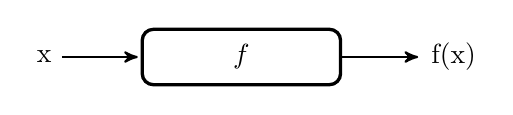
\begin{tikzpicture}[->,>=stealth',shorten >=1pt,auto,node distance=1cm,
      thick,main node/.style={circle,fill=blue!20,draw,font=\sffamily\Large\bfseries}]
    \node[punkt] (natur) {$f$};
    \node[left=of natur] (x) {x};
    \node[right=of natur] (y) {f(x)};
    \path[every node/.style={font=\sffamily\small}]
    (natur) edge node {} (y)
    (x) edge node  {} (natur)
    ;
  \end{tikzpicture}
\end{center}

  predicted outcomes are very close to real targets: $\fx \approx y$

\end{itemize}

\begin{itemize}

\item
  We call this \textbf{supervised learning}.
\end{itemize}

\end{frame}

\begin{frame}{What is a Model?}

%A model takes the features of new observations and produces a prediction
%\(\hat{y}\) of our target variable \(y\):

A model (or hypothesis) $f : \Xspace \rightarrow \R^g$ maps inputs (or input features) to outputs (or targets).

A hypothesis class $H$ is a set of such functions.

\scriptsize

\begin{center}\includegraphics[width=0.9\textwidth]{plots/the_model_web} \end{center}

\normalsize 

\end{frame}

\begin{frame}{What is a Learner?}

The \textbf{learner} (inducer, learning algorithm) takes our labeled data set
(\textbf{training set}) and produces a model (which again is a
function):

Applying a learning algorithm means coming up with a hypothesis given sample data. 
Formally, it maps:
$$\{((x^{(1)},y^{(1)}),...,(x^{(n)},y^{(n)}))\} \subset \Xspace \times \Yspace \rightarrow \Hspace$$

\vspace{-0.5cm}

\scriptsize

\begin{center}\includegraphics[width=0.7\textwidth]{plots/the_inducer_web} \end{center}

\normalsize 

\end{frame}

\begin{frame}{How to Evaluate Models}

\begin{itemize}

\item
  Simply compare predictions from model with truth:
\end{itemize}

\scriptsize

\begin{center}\includegraphics[width=0.8\textwidth]{plots/eval_inducer1_web} \end{center}

\normalsize 
\end{frame}

\begin{frame}{Learner Decomposition}

Nearly all ML supervised learning training algorithms can be described
by three components:

\begin{center}
  \textbf{Learning = Hypothesis Space + Evaluation + Optimization}
\end{center}

\begin{itemize}
\item
  \textbf{Hypothesis Space:} Defines functional
  structures of \(f\) we can learn.
\item
  \textbf{Evaluation:} How well does a certain hypothesis score on a
  given data set? Allows us to choose better candidates over worse ones.
\item
  \textbf{Optimization:} How do we search the hypothesis space? Guided
  by the evaluation metric.
\item
  All of these components represent important choices in ML which can
  have drastic effects:
  \newline
  If we make smart choices here, we can tailor our learner to our needs
  - but that usually requires quite a lot of experience and deeper
  insights into ML.
\end{itemize}

\end{frame}

\begin{frame}{Learner Decomposition}

\begin{table}[]
\begin{tabular}{lllll}
  \textbf{Hypothesis Space} & \textbf{Evaluation} &  \textbf{Optimization}&  &  \\
Instances / Neighbours & Squared error & Gradient descent &  \\
Linear functions & Likelihood & Stochastic gradient descent  &  \\
Decision trees & Information gain & Quadratic programming & \\
Set of rules & K-L divergence & Greedy optimization & \\
Neural networks & & Combinatorial optimization & \\
Graphical models & & \\
\end{tabular}
\end{table}

Note: What is on the same line above does not belong together!

\end{frame}


\begin{vbframe}{Risk minimization}

Let \(\mathbb P_{xy}\) be the joint distribution of \(x\) and \(y\).
  This defines all aspects of the generating process where our data
  comes from. 
\vfill
The quality of the prediction $y=\fx$ of a model is measured by a \emph{loss function} $\Lxy $.
\vfill
A function $L :\Yspace \times \Yspace \rightarrow [0, \infty[$ with the property $L(y, y) = 0$ for $y \in  \Yspace$ is called a loss function.
\vfill
A typical loss function is the squared error: $\Lxy = (y-\fxt)^2$,
\vfill
Its expectation is the so-called \emph{risk},
  $$ \riskf = \E [\Lxy] = \int \Lxy d\Pxy. $$
\vfill
 Obvious aim: Minimize $\riskf$ over $f$. 
  
\framebreak
  
But minimizing $\riskf$ over $f$ is not (in general) practical:

\begin{itemize}
\item $\Pxy$ is unknown.
\item We could estimate $\Pxy$ in non-parametric fashion from the data $D$, e.g., by kernel density
  estimation, but this really does not scale to higher dimensions (see curse of dimensionality).
\item We can efficiently estimate $\Pxy$, if we place rigorous assumptions on its distributional form,
  and methods like discriminant analysis work exactly this way. ML usually studies more flexible models.
\end{itemize}


\framebreak

An alternative (without directly assuming something about $\P_{xy}$) is to approximate $\riskf$ based on
the data $\D$, by means of the \emph{empirical risk}

$$
\riske(f) = \frac{1}{n} \sumin \Lxyi
$$

Learning then amounts to \emph{empirical risk minimization}
$$
\fh = \argmin_{f \in \Hspace} \riske(f).
$$

\framebreak

When $f$ is parameterized by $\theta$, this becomes:

\begin{eqnarray*}
\riske(\theta) & = & \frac{1}{n} \sumin \Lxyit \cr
\hat{\theta} & = & \argmin_{\theta \in \Theta} \riske(\theta)
\end{eqnarray*}

Thus learning (often) means solving the above \emph{optimization problem}.
Which implies a tight connection between ML and optimization.

Note that (with a slight abuse of notation), if it is more convenient, and as there is no difference w.r.t.
the minimizer, we might also define the $\riske$ in its non-average-but-instead-summed version as:

$$
\risket = \sumin \Lxyit
$$

\framebreak

\begin{itemize}
\item For regression, the loss usually only depends on residuals: $\Lxy = L(y - \fx) = L(\eps)$,
  this is a \emph{translation invariant} loss
\item Choice of loss decides statistical properties of $f$: Robustness, error distribution
\item Choice of loss decides computational / optimization properties of minimization of $\risket$:
  Smoothness of objective, can gradient methods be applied, uni- or multimodality. \\
  If $\Lxy$ is convex in its second arguments, and $\fxt$ is linear in $\theta$, then $\risket$ is convex.
  Hence every local minimum of $\risket$ is a global one. If $\Lxy$ not convex,
  R might have multiple local minima (bad!).
\end{itemize}
\end{vbframe}

\section{(Linear) Regression}

\begin{frame}{Straight Line / Univariate Linear Model}

\scriptsize

\begin{center}
\includegraphics[width=0.7\textwidth]{plots/straight-line.png}
\end{center}


\normalsize 

\[
y = \theta_0 + \theta \cdot x
\]

\end{frame}

\begin{frame}{Linear Regression: Hypothesis Space}

We want to learn a numerical target variable, by a linear transformation
of the features. So with \(\theta \in \mathbb{R}^p\) this mapping can be
written: \[
y = \fx = \theta_0 + \theta^T x
\]

This restricts the hypothesis space \(H\) to all linear functions in
\(\theta\): \[
H = \{ \theta_0 + \theta^T x\ |\ (\theta_0, \theta) \in \mathbb{R}^{p+1} \}
\]

Given observed labeled data \(\D\), how to find \((\theta, \theta_0\))?
This is learning or parameter estimation.

NB: We assume here and from now on that \(\theta_0\) is included in
\(\theta\).

\end{frame}

\begin{frame}{Linear Regression: Evaluation}

We now measure training error as sum-of-squared errors. This is also
called the L2 loss, or L2 risk: \[
\risket = \operatorname{SSE}(\theta) = \sumin \Lxyit = \sumin \left(\yi - \theta^T \xi\right)^2
\]

\scriptsize

\begin{center}
\includegraphics[width=0.6\textwidth]{plots/lin-reg.png}
\end{center}


\normalsize  \vspace{-0.4cm} Optimizing the squared error is
computationally much simpler than optimizing the absolute differences
(this would be called L1 loss).

\end{frame}


\begin{frame}{Linear Regression: Optimization}

We want to find the parameters of the LM / an element of the hypothesis
space H that best suits the data. So we evaluate different candidates
for \(\theta\).

\begin{itemize}
\item
  A first (random) try yields an SSE of 20.33 (\textbf{Evaluation}).
\end{itemize}

\begin{center}
\includegraphics[width=0.6\textwidth]{plots/lin-reg-optim01.png}
\end{center}


\end{frame}


\begin{frame}{Linear Regression: Optimization}

We want to find the parameters of the LM / an element of the hypothesis
space H that best suits the data. So we evaluate different candidates
for \(\theta\).

\begin{itemize}
\item
  Another line yields an lower SSE of 18.51 (\textbf{Evaluation}).
\end{itemize}

\begin{center}
\includegraphics[width=0.6\textwidth]{plots/lin-reg-optim02.png}
\end{center}

\end{frame}

\begin{frame}{Linear Regression: Optimization}

Instead of guessing parameters we could also use gradient descent to
iteratively find the optimal \(\theta\). Here, we can even find the
optimal value analytically: \[
\hat{\theta} = \argmin_{\theta} \risket = \argmin_{\theta} \|y - X\theta\|^2_2
\] \(X\) is the \(n \times (p+1)\)-feature-data-matrix, also called
design matrix.

This yields the so called normal equations for the LM: \[
\frac{\delta}{\delta\theta} \risket = 0 \qquad \Rightarrow\ \qquad \hat{\theta} = \left(X^T X\right)^{-1}X^Ty
\]

\end{frame}



\begin{vbframe}{Linear Regression: Optimization}

Differentiating $\risket = \operatorname{SSE}(\theta)$ w.r.t $\theta$ yields the so-called \emph{normal equations}:
$$
X^T(\ydat - X\theta) = 0
$$
The optimal $\theta$ is
$$
\thetah = (X^T X)^{-1} X^T\ydat
$$

\framebreak

The optimal line has an SSE of 9.77 (\textbf{Evaluation})

\begin{center}
\includegraphics[width=0.7\textwidth]{plots/lin-reg-optim03.png}
\end{center}

\framebreak

In statistics, we would start from a maximum-likelihood perspective
$$
\yi = \fxi + \epsi \sim N(\fxi, \sigma^2)
$$
$$
\LLt = \prod_{i=1}^n \pdf(\yi | \fxit, \sigma^2) \propto \exp(-\frac{\sumin (\fxit - \yi)^2}{2\sigma^2})
$$
If we minimize the neg. log-likelihood, we see that this is equivalent to our
loss minimization approach!
$$
\llt \propto \sumin (\fxit - \yi)^2  = min!
$$
\end{vbframe}


\begin{frame}{Example: Linear Regr. With L1 vs L2 Loss}

We could also minimize the L1 loss. This changes the evaluation and
optimization step: \[
\risket = \sumin \Lxyit = \sumin |\yi - \theta^T \xi| \qquad \textsf{(Evaluation)}
\] Much harder to optimize, but the model is less sensitive to outliers.

\scriptsize

\begin{center}
\includegraphics[width=0.7\textwidth]{plots/lin-reg-L1.png}
\end{center}

\normalsize 

\end{frame}

\begin{frame}{Example: Linear Regr. With L1 vs L2 Loss}

Adding an outlier (highlighted red) pulls the line fitted with L2 into
the direction of the outlier:

\scriptsize
\begin{center}
\includegraphics[width=0.8\textwidth]{plots/example-lin-reg.png}
\end{center}

\normalsize 

\end{frame}


\section{Classification}

\begin{frame}{Binary Classification Task}

\begin{itemize}
\item
  \(y\) is a categorical variable (with two values)
\item
  E.g., sick/healthy, or credit/no credit
\item
  \textbf{Goal}: Predict a class (or membership probabilities)
\end{itemize}

\scriptsize
\begin{center}
\includegraphics[width=0.8\textwidth]{plots/binary-class.png}
\end{center}


\normalsize 

\end{frame}

\begin{frame}{Multiclass Classification Task}

\begin{itemize}
\item
  \(y\) is a categorical variable with \textgreater{} 2 unordered values
\item
  Each instance belongs to only one class
\item
  \textbf{Goal}: Predict a class (or membership probabilities)
\end{itemize}

\scriptsize

\begin{center}
\includegraphics[width=0.8\textwidth]{plots/multi-class.png}
\end{center}

\normalsize 

\end{frame}

\begin{frame}{Classification: Posterior Probabilities}

\begin{itemize}
\item
  Often estimating class probabilities for observations is more
  informative than predicting labels.
\item
  Posterior probabilities are the probability of a class \(k\) occuring,
  given the feature \(x\) \[
  \pikx = P(Y = k | x)
  \]
\item
  Many models can directly output and optimize for these probabilities.
\item
  Class estimation for \(x\) via \(\argmax_{k} \pikx\) - just take most
  likely class.
\end{itemize}

\end{frame}

\begin{frame}{Classification: Decision Boundary}

\begin{itemize}
\item
  Area in feature space where there is no unique best class with maximum
  posterior probability are equal, e.g., for binary classification
  \(\pix_1 = \pix_2\)
\item
  Separates areas in which a specific class is estimated / chosen.
\end{itemize}

\scriptsize
\begin{center}
\includegraphics[width=0.8\textwidth]{plots/decision-boundary.png}
\end{center}

\normalsize 

\end{frame}



\begin{vbframe}{Binary label coding}

\remark{
Notation in binary classification can be sometimes confusing because of different coding styles,
and as we have to talk about predicted scores, classes and probabilities.
}

\lz

A binary variable can take only two possible values.
For probability / likelihood-based model derivations a 0-1-coding, for geometric / loss-based models
the -1+1-coding is often preferred.

\begin{itemize}
\item $\Yspace = \{0, 1\}$. Here, the approach often models $\pix$, the posterior probability for class 1 given $x$.
  Usually, we then define $\hx = [\pix \geq 0.5] \in \Yspace$.
\item $\Yspace = \{-1, 1\}$. Here, the approach often models $\fx$, a real-valued score from $\R$ given x.
  Usually, we define $\hx = \sign(\fx) \in \Yspace$, and we interpret
  $|\fx|$ as \enquote{confidence} for the predicted class $\hx$.
\end{itemize}

\lz


\end{vbframe}


\begin{vbframe}{Logistic regression}

A \emph{discriminant} approach for directly modeling the posterior probabilities of the classes is \emph{Logistic regression}. For now, we will only look at the binary case $y \in \{0, 1\}$.
Note that we will supress the intercept in notation.

$$
\pix = \post = \frac{\exp(\theta^Tx)}{1+\exp(\theta^Tx)} = \tau(\theta^T x)
$$

We can either directly assume the above form, or arrive at it by requiring that the log-odds
are linear in $\theta$:

$$
\log \frac{\pix}{1-\pix} = \log\frac{\post}{\P(y = 0 | x)} = \theta^Tx.
$$\

\lz

The logistic function $\tau(t) = \frac{\exp(t)}{1 + \exp(t)}$
transforms the scores / log-odds $\theta^Tx$ into a probability.



\framebreak

Logistic regression is usually fitted by maximum likelihood.
\begin{eqnarray*}
\LLt &=& \prod_{i=1}^n \P(y = y^{(i)} | x^{(i)}, \theta) \\
% &=& \prod_{i=1}^n (\P(y = 1 | x^{(i)}, \theta)^{y^{(i)}}[1 - \P(y = 1 | x^{(i)}, \theta)]^{1 - y^{(i)}} \\
&=& \prod_{i=1}^n \pi(x^{(i)}, \theta)^{y^{(i)}} [1 - \pi(x^{(i)}, \theta)]^{1 - y^{(i)}}.
\end{eqnarray*}

% \framebreak

% Consequently, the log-likelihood is derived by

\small
\begin{eqnarray*}
\llt
&=& \sum_{i=1}^n \yi \log[\pi(\xi, \theta)] + (1-\yi) \log [1 - \pi(\xi, \theta)]\\
&=& \sum_{i=1}^n \yi \log [\exp(\theta^T \xi)] - \yi \log[1 + \exp(\theta^T \xi)] \\
&\quad& + \quad (1 - \yi) \log \biggl[1 - \frac{\exp(\theta^T \xi)}{1 + \exp(\theta^T \xi)}\biggr]\\
&=& \sum_{i=1}^n \yi \theta^T \xi - \log[1 + \exp(\theta^T \xi)]
\end{eqnarray*}

\framebreak

\normalsize
We can minimize our loss, by maximizing $\llt$.
% Therefore, we need to differentiate w.r.t. $\theta$, which gives us the score function:\\
% $$
% s(\theta) = \fp{\llt}{\theta} = \sum_{i=1}^n \xi \cdot \left( \yi - \frac{\exp(\theta^T \xi)}{1 + \exp(\theta^T \xi)}\right) = 0
% $$

% \lz

This now cannot be solved analytically, but is at least concave, so we have to refer to numerical optimization, e.g., gradient ascent.

\lz

To predicted class labels with minimal errors, we should probably predict $y=1$, iff

$$
\pixt = \frac{\exp(\theta^T x)}{1+\exp(\theta^Tx)} \ge 0.5,
$$

which is equal to
$$
\theta^T x \ge 0.
$$

So logistic regression gives us a \emph{linear classifier}:
$$
\yh = h(\theta^T x) =
\begin{cases}
1 & \text{ for } x^T\theta \ge 0 \\
0 & \text{ otherwise}
\end{cases}
$$


\framebreak

\begin{center}
\includegraphics[width=0.9\textwidth]{plots/logistic-reg.png}
\end{center}

\end{vbframe}

\begin{frame} {Types of boundaries that can be learned}
  \begin{itemize}
    \item Different values of $\theta$ map to different linear decision boundaries separating the two classes.
    \vspace{5mm}
    \begin{figure}
    \centering
      \scalebox{1}{\includegraphics{plots/lin_bound.png}}
  \end{figure}
    \vspace{5mm}
  Note : Only two dimensions pictured here
  \end{itemize}
\end{frame}

\begin{frame} {Types of boundaries that can be learned}
\begin{itemize}
  \item The intercept $\theta_0$, is in ML often (unfortunately) called bias.
    \item It produces an affine shift on the linear decision boundary.
    % Deeplearningbook page 110: This terminology derives from the point of view that the output of the transformation is biased toward being b in the absence of any input.
  \end{itemize}
    \begin{figure}
      \centering
        \includegraphics[width=8.5cm]{plots/bias.png}
    \end{figure}
\end{frame}

\begin{vbframe}{Likelihood and losses}

Let us generalize what we have observed from the comparison between the maximum-likelihood and the risk-based approach linear regression.

The maximum-likelihood principle is to maximize
$$ \LLt = \prod_{i=1}^n \pdfyigxit $$
or to minimize the neg. log-likelihood:
$$ -\llt = -\sumin \lpdfyigxit $$
Now let us define a new loss as:
$$ \Lxyt = - \lpdfygxt $$
And consider the empirical risk
$$\risket = \sumin \Lxyt$$

Then the maximum-likelihood estimator $\thetah$, which we obtain by optimizing $\LLt$ is identical
to the loss-minimal $\thetah$ we obtain by minimizing $\risket$.
This implies that we can identify for every error distribution and its pdf $\pdfygxt$ an
equivalent loss function which leads to the same point estimator for the parameter vector $\theta$.
We can even disregard multiplicative or additive constants in the loss,
as they do not change the minimizer.

The other way around does not always work: We cannot identify for every loss function and associated pdf for the distribution. 

\framebreak

Let us reconsider the logistic regression maximum likelihood fit. The neg. log-likelihood for the pdf is:

$$
-\lpdfygxt = - y \log[\pix] - (1-y) \log [1 - \pix]
$$

This is the cross-entropy loss. Logistic regression minimizes this, and we could use this loss for any other model which directly models $\pix$.

\lz

Now lets assume we have a score function $\fx$ instead of $\pix$. We can transform the score to a probability via the logistic transformation:

\begin{eqnarray*}
\pix     &=& \frac{\exp(\fx)}{1 + \exp(\fx)}   =  \frac{1}{1 + \exp(-\fx)}\\
1- \pix  &=& \frac{\exp(-\fx)}{1 + \exp(-\fx)} =  \frac{1}{1 + \exp(\fx)}\\
\end{eqnarray*}

\framebreak

The loss now becomes
\begin{eqnarray*}
-\lpdfygxt &=& -y \log[\pix] - (1-y) \log [1 - \pix] \\
           &=& y \log[1 + \exp(-\fx)] + (1-y) \log[1 + \exp(\fx] \\
\end{eqnarray*}
For y=0 and y=1 this is:
\begin{eqnarray*}
y=0 &:& \log[1 + \exp(\fx] \\
y=1 &:& \log[1 + \exp(-\fx)]
\end{eqnarray*}
If we would encode now with $\Yspace = \{-1,+1\}$, we can unify this like this:
$$\Lxy = \log[1 + \exp(-\yf] $$
So we have recovered the Bernoulli loss. LR minimizes this, and we could use this loss for any other model with directly models $\fx$.

\end{vbframe}



\begin{vbframe}{Estimating Probabilities}

In logistic regression, the logistic function transforms the log-odds $t = \theta^Tx$ into a probability:
$\tau(t) = \frac{\exp(t)}{1 + \exp(t)}$.\\
\lz
$\tau(t)$ is a so-called sigmoid function.
The above approach can be generalized, so other score-generating models $\fx$ can be turned into
probability estimators by using $\tau(f(x))$.

\begin{itemize}
\item $f$ could be another model that outputs a score
\item $\tau$ could be another sigmoid-function (i.e. the cdf of the standard normal distribution which leads to the \emph{probit}-model)
\item We have to choose an appropriate loss, e.g. binomial or cross-entropy loss.
  One (older) approach is also to simply use $\tau(f(x))$ as the model and then minimize the squared loss
  between $\yh$ and the $(0,1)$ labels.
\end{itemize}
\end{vbframe}

\begin{vbframe}{Estimating Probabilities - Sigmoid}

  A \emph{sigmoid} is a bounded, differentiable, real-valued function $\tau: \R \to (0,1)$, that has a non-neg. derivative at each point.
\lz

  Properties of logistic function $\tau(t)$:
\begin{itemize}
\item $\lim_{t \to\ -\infty} \tau(t) = 0$ and  $\lim_{t \to \infty} \tau(t) = 1$
\item $\fp {\tau(t)}{t}=\frac{\exp(t)}{(1+\exp(t))^2} = \tau(t)(1-\tau(t))$
\item $\tau(t)$ is symmetrical about the point $(0, 1/2)$
\end{itemize}

\begin{center}
\includegraphics[width=0.9\textwidth]{plots/sigmoid.png}
\end{center}

\framebreak

\end{vbframe}

\begin{vbframe}{Multinomial Regression and Softmax}

For a categorical response variable $y \in \gset$ with $g>2$ the model extends to

$$
\pikx = \P(y = k | x) = \frac{\exp(\theta_k^Tx)}{\sum_{j=1}^g\exp(\theta_j^Tx)}.
$$

The latter function is called the \emph{softmax}, and defined on a numerical vector $z$:
$$
\tau(z)_k = \frac{\exp(z_k)}{\sum_{j}\exp(z_j)}
$$

It is a generalization of the logistic function (check for g=2). It \enquote{squashes} a g-dim. real-valued vector $z$ to a vector of the same dimension,
with every entry in the range [0, 1] and all entries adding up to 1.

\framebreak

By comparing the posterior probabilities of two categories $k$ and $l$ we end up in a linear function (in $x$),

$$
\log\frac{\pi_k(x)}{\pi_l(x)} = (\theta_k-\theta_l)^Tx.
$$

\textbf{Remark:}
\begin{itemize}
\item $\theta_j$ are vectors here.
\item Well-definedness: $\pi_k(x) \in [0, 1]$ and $\sum_k \pi_k(x) = 1$

\end{itemize}

\framebreak

This approach can be extended in exactly the same fashion for other score based models.
For each class $k$ we define a binary score model $f_k(x)$ with parameter vector $\theta_k$.
We then combine these models through the softmax function

$$
\postk = \pikx = s_k(f_1(x), \ldots f_g(x))
$$

and optimize all parameter vectors of the $f_k$ jointly. Maximum likelihood:

$$
\LLt = \prodin \prodkg \pikxt^{[y = k]}
$$

Negative log-likelihood turns this into empirical risk minimization:

$$
\risket = \sumin \sumkg 1_{[y = k]} \log s_k(f_1(x | \theta_k), \ldots f_g(x | \theta_g))
$$

\framebreak

Further comments:

\begin{itemize}

\item We can now, e.g., calculate gradients and optimize this with standard numerical optimization software.

\item For linear $\fxt = \theta^T x$ this is also called \emph{softmax regression}.

\item Has an unusual property that it has a \enquote{redundant} set of parameters. If we substract a fixed vector
  from all $\theta_k$, the predictions do not change at all.
  I.e.,  our model is \enquote{overparameterized}, and for any hypothesis we might fit,
  there are multiple parameter vectors that give rise to exactly the same hypothesis function.
  This also implies that the minimizer of $\risket$ above is not unique (but $\risket$ is convex)!
  Hence, a numerical trick is to set $\theta_g = 0$ and only optimize the other $\theta_k$.

\item A similar approach is used in many ML models: multiclass LDA, naive Bayes, neural networks and boosting.

\end{itemize}

\end{vbframe}



%%%%%%%%%%%%%%%%%%%%%%%%%%%%%%%%%%%%%%%%%%%%%
%%%%%%%%%%%%%%%%%%%%%%%%%%%%%%%%%%%%%%%%%%%%
%%%%%%%%%%%%%%%%%%%%%%%%%%%%%%%%%%%%%%%%%%%%
%%%%%%%%%%%%%%%%%%%%%%%%%%%%%%%%%%%%%%%%%%%



\section{Performance Measures and Generalization}

\begin{frame}{Overfitting}

\begin{itemize}
\item
  Learner finds a pattern in the data that is not actually true in the
  real world: \emph{overfits} the data
\item
  Every powerful learner can \enquote{hallucinate} patterns
\item
  Happens when you have too many hypotheses and not enough data to tell
  them apart
\item
  The more data, the more \enquote{bad} hypotheses are eliminated
\item
  If the hypothesis space is not constrained, there may never be enough
  data
\item
  There is often a parameter that allows you to constrain
  (\emph{regularize}) the learner
\end{itemize}

\end{frame}

\begin{frame}{Overfitting}

\begin{columns}[T,onlytextwidth]
\column{0.5\textwidth}
Overfitting learner \\
\vspace{0.5cm}

\scriptsize

\begin{center}
\includegraphics[width=0.9\textwidth]{plots/overfitting-learner.png}
\end{center}

\normalsize 
Better training set performance (seen examples)

\column{0.5\textwidth}
Non-overfitting learner \\
\vspace{0.5cm}

 \scriptsize
\begin{center}
\includegraphics[width=0.9\textwidth]{plots/non-overfitting-learner.png}
\end{center}

 \normalsize 
Better test set performance (unseen examples)
\end{columns}

\end{frame}

\begin{frame}{Overfitting and Noise}

\begin{itemize}
\item
  Overfitting is seriously exacerbated by \emph{noise} (errors in the
  training data)
\item
  An unconstrained learner will start to model that noise
\item
  It can also arise when relevant features are missing in the data
\item
  In general it's better to make some mistakes on training data
  (\enquote{ignore some observations}) than trying to get all correct
\item
  To avoid overfitting:  
  \begin{itemize}
    \item
      Some learners can do \enquote{early stopping} before perfectly fitting
      (i.e., overfitting) the training data
    \item
      In general, prefer simpler hypotheses altogether when they work well
      (e.g.~regularization, pruning)
  \end{itemize}
\end{itemize}

\end{frame}

\begin{frame}{Triple Trade-Off}

In all learning algorithms that are trained from data, there is a
trade-off between three factors:

\begin{itemize}
\item
  The complexity of the hypothesis we fit to the training data
\item
  The amount of training data (in terms of both instances and
  informative features)
\item
  The generalization error on new examples
\end{itemize}

If the capacity of the learning algorithm is large enough to a)
approximate the data generating process and b) exploit the information
contained in the data, the generalization error will decrease as the
amount of training data increases.

For a fixed size of training data, the generalization error decreases
first and then starts to increase (overfitting) as the complexity of the
hypothesis space \(H\) increases.

\end{frame}

\begin{frame}{Trade-Off Between Generalization Error and Complexity}

Apparent error (on the training data) and real error (prediction error
on new data) evolve in the opposite direction with increasing
complexity:

\scriptsize

\begin{center}
\includegraphics[width=0.8\textwidth]{plots/trade-off.png}
\end{center}

\normalsize  \vspace{-0.2cm} \(\Rightarrow\) Optimization regarding the
model complexity is desirable: Find the right amount of complexity for
the given amount of data where generalization error becomes minimal.

\end{frame}



%
% \begin{vbframe}{Risk minimizing functions}
%
% Overview of binary classification losses and the corresponding risk minimizing functions:
%
% \lz
%
% \begin{tabular}{p{2.5cm}|p{3.5cm}|p{4.5cm}}
%   loss name & loss formula  & minimizing function \\
%   \hline
%   0-1 & $[y \neq \hx]$ & $\hxh = \footnotesize \begin{cases} 1 \quad \text{ if } \pix > 1/2 \\ -1 \quad \pix < 1/2  \end{cases}$ \\
%   Hinge & $\max\{0, 1 - \yf\}$ & $\fh(x) =  \footnotesize \begin{cases} 1 \quad \text{ if } \pix > 1/2 \\ -1 \quad \pix < 1/2  \end{cases}$ \\
%   Logistic & $\ln(1+\exp(-y\fx))$ & $\fh(x) =  \ln \biggl(\frac{\pix}{1-\pix}\biggr)$ \\
%   Cross entropy & $-y\ln(\pix) \newline -(1-y)\ln(1-\pix)$ & \\
%   & & \\
%   Exponential & $\exp(-y\fx)$ &
%
% \end{tabular}
%
% \end{vbframe}

% \section{Selected methods for regression and classification}


\begin{frame}{Performance Measures}

\begin{centering}
\includegraphics[width=9cm,page=1]{plots/make_classif_regr_error_intro_plot.pdf}
\end{centering}

To compare the performance of two ML models on a single observation or a
new data set, we would ideally like to boil them down to a
\textbf{single} numeric measure of the performance.

\end{frame}

\begin{frame}{Performance Measures}


Performance measures are related to losses, but are not the same.

\begin{itemize}

\item A performance measure is simply applied at the end, to a fitted model, and some 
  test data under consideration. A loss function is optimized by a learning algorithm.

\item A performance measure is usually dictated by our prediction problem. There are no technical 
  restrictions on it, except that it needs to be computable and appropriate, as it is only
  measured on a model and data set, to evaluate the model.
  A loss function on the other hand needs to be \enquote{handable} by the optimizer, so a certain
  degree of smoothness is usually required.

\item Sometimes, performance mearures arer called \enquote{outer losses},
  and \enquote{innner loss} is used for the loss minimized by the learner.

\item Sometime, one can make the inner loss match the outer loss, so the learning algorithm 
  optimizes exactly the metric we are interested in. But often we use approximations for the
  inner loss, e.g., for efficiency.

\end{itemize}

\end{frame}


\begin{frame}{Regression: MSE}

The \textbf{Mean Squared Error} compares the mean of the squared
distances between the target variable \(y\) and the predicted target
\(\yh\). \[
MSE = \frac{1}{n} \sumin (\yi - \yih)^2 \in [0;\infty]
\]

Single observations with a large prediction error heavily influence the
\textbf{MSE}, as they enter quadratically.

\scriptsize

\begin{center}
\includegraphics[width=0.7\textwidth]{plots/MSE.png}
\end{center}

\normalsize 

\end{frame}

\begin{frame}{Regression: MAE}

A more robust (but not neccessarily better) way to compute a performance
measure is the \textbf{Mean Absolute Error}:

\[
MAE = \frac{1}{n} \sumin |\yi - \yih| \in [0;\infty]
\]

The absolute error is more robust. On the other hand, the absolute error
is not differentiable at \(0\).

\scriptsize

\begin{center}
\includegraphics[width=0.7\textwidth]{plots/MAE.png}
\end{center}

\normalsize 

\end{frame}

\begin{frame}{Regression: \(R^2\)}

Another often used measure is \(R^2\). It measures the \emph{fraction of
variance explained} by the model. \[
R^2 = 1 - \frac{\sumin (\yi - \yih)^2}{\sumin (\yi - \bar{y})^2} = \frac{SSE_{Model}}{SSE_{Intercept}}
\]

\begin{itemize}
\item
  If \(R^2\) is measured on the training data: \(R^2 \in [0;1]\).
\item
  If \(R^2\) is measured on held out data: \(R^2 \in [-\infty;1]\).
\end{itemize}

\end{frame}

\begin{frame}{Regression: Defining a custom loss}

Assume a use case, where the target variable can have a wide range of
values across different orders of magnitude. A possible solution would
be to use a loss functions that allows for better model evaluation and
comparison. The \textbf{Mean Squared Logarithmic Absolute Error} is not
strongly influenced by large values due to the logarithm. \[
\frac{1}{n} \sumin (\log(|\yi - \yih| + 1))^2
\]

\scriptsize
\begin{center}
\includegraphics[width=0.7\textwidth]{plots/custom-loss.png}
\end{center}

\normalsize 

\end{frame}

\begin{frame}{Performance Measures - Classification}

The confusion matrix is an intuitive metric used for establishing the
correctness and accuracy of a model. It is used for classification
problems where the output can be of two or more types of classes.
\newline
\begin{centering}
\includegraphics[width=10cm,page=3]{plots/confusion_matrix_measures.pdf}
\end{centering}

\end{frame}

\begin{frame}{Classification: Accuracy / Error}

The confusion matrix is not a performance measure as such, but most
performance metrics for binary classification are based on it.
\newline
\begin{centering}
\includegraphics[width=10cm,page=4]{plots/confusion_matrix_measures.pdf}
\end{centering}

Classification Error = 1 - Accuracy

\end{frame}

\begin{frame}{Threshold}

Thresholding flexibly converts measured probabilities to labels.

\begin{centering}
\includegraphics[height=8cm, width=14cm,page=2]{plots/confusion_matrix_measures.pdf}
\end{centering}

\end{frame}

\begin{frame}{Classification Performance Measures}

\small

\begin{table}[]
\begin{tabular}{ll}
\hline
\textbf{Classification}& \textbf{Explanation}  \\ \hline
Accuracy              &  Fraction of correct classifications                             \\ \hline
Balanced Accuracy     &  Fraction of correct classifications in each class               \\ \hline
Recall                &  Fraction of positives a classifier captures                     \\ \hline
Precision             &  Fraction of positives in instances predicted as positive        \\ \hline 
F1-Score              &  Tradeoff between precision and recall                           \\ \hline
AUC                   &  Measures calibration of predicted Probabilities                 \\ \hline
Brier Score           &  Squared difference between predicted probability                \\ 
                      & and true label                                                   \\ \hline
Logloss               &  Emphasizes errors for predicted probabilities close             \\ 
                      & to 0 and 1                                                       \\ \hline
\end{tabular}
\end{table}

\normalsize

\end{frame}

\begin{frame}{Training Error}

The \emph{training error} (also called apparent error or resubstitution
error) is estimated by the average error over the training set
\(\Dtrain\):

\includegraphics[width=12cm,page=4]{plots/train_error.png}

\end{frame}

\begin{frame}{Training Error}

\begin{itemize}
\item
  The training error is usually a very unreliable and overly optimistic
  estimator of future performance.
\item
  Goodness-of-fit measures like \(R^2\), likelihood, AIC, BIC, deviance
  are all based on the training error.
\end{itemize}

\end{frame}

\begin{frame}{Example: Polynomial Regression}

Assume we have a single, univariate \(x\) and that \(y\) can be
approximated by a \(d\)th-order polynomial

\[ \fxt = \theta_0 + \theta_1 x + \cdots + \theta_d x^d = \sum_{j = 0}^{d} \theta_j x^j\text{.} \]

\(\theta_j\) are the coefficients and \(d\) is called the degree.

This is still linear regression / a linear model, and for a fixed \(d\),
the \(\theta\) can easily be obtained through the normal equations.

\end{frame}

\begin{frame}{Example: Polynomial Regression}

True relationship is
\(f(x) = 0.5 + 0.4 \cdot \sin (2 \pi x) + \epsilon\)

\scriptsize
\begin{center}
\includegraphics[width=0.9\textwidth]{plots/poly-reg01.png}
\end{center}

\normalsize 

\end{frame}

\begin{frame}{Example: Polynomial Regression}

Models of different \emph{complexity}, i.e., of different orders of the
polynomial are fitted. How should we choose \(d\)?

\scriptsize

\begin{center}
\includegraphics[width=0.9\textwidth]{plots/poly-reg02.png}
\end{center}

\normalsize 

\end{frame}

\begin{frame}{Example: Polynomial regression}

The performance of the models on the training data can be measured by
calculating the \emph{training error} according to the mean squared
error (MSE) criterion:

\[ \frac{1}{n} \sum_{i = 1}^{n}(y_i - \hat{y}_i)^2\text{.} \]

d = 1: 0.03, \qquad d = 5: 0.002, \qquad d = 9: 0.001

Simply using the training error seems to be a bad idea.

\end{frame}

\begin{frame}{Training Error Problems}

\begin{itemize}
\item
  Extend any ML training in the following way: On top of normal fitting,
  we also store \(\Dtrain\). During prediction, we first check whether
  \(x\) is already stored in this set. If so, we replicate its label.
  The training error of such an (unreasonable) procedure will always be
  zero.
\item
  The training error of 1-NN is always zero.
\item
  The training error of an interpolating spline in regression is always
  zero.
\item
  For models of severely restricted capacity, and given enough data, the
  training error might provide reliable information. E.g. consider a
  linear model in 5d, with 10.000 training points. But: What happens if
  we have less data? And \(p\) becomes larger? Can you precisely define
  where the training error becomes unreliable?
\end{itemize}

\end{frame}

\begin{frame}{Test Error and Hold-Out Splitting}

To reliably assess a model, we need to define

\begin{itemize}
\item
  how to simulate the scenario of \enquote{new unseen data} and
\item
  how to estimate the generalization error.
\end{itemize}

Hold-out splitting and evaluation

\begin{itemize}
\item
  Straightforward idea: To measure performance, let's simulate how our
  model will be applied on new, unseen data
\item
  So, to evaluate a given model: predict and evaluate only on data not
  used during training
\item
  For a given set \(\D\), we have to preserve some data for testing that
  we cannot use for training, hence we need to define a training set
  \(\Dtrain\) and a test set \(\Dtest\), e.g.~by randomly partitioning
  the original \(\D\)
\end{itemize}

\end{frame}

\begin{frame}{Test Error and Hold-Out Splitting}

\includegraphics[width=11cm]{plots/test_error.png}

\end{frame}

\begin{frame}{Test Error and Hold-Out Splitting}

\scriptsize

\begin{center}
\includegraphics[width=0.9\textwidth]{plots/test_error01.png}
\end{center}

\normalsize 

\end{frame}

\begin{frame}{Test Error and Hold-Out Splitting}

\scriptsize

\begin{center}
\includegraphics[width=0.9\textwidth]{plots/test_error02.png}
\end{center}

\normalsize 

\end{frame}

\begin{frame}{Test Error and Hold-Out Splitting}

\scriptsize

\begin{center}
\includegraphics[width=0.9\textwidth]{plots/test_error03.png}
\end{center}

\normalsize  Test error is best for \(d=3\)

\end{frame}

\begin{frame}{Training vs.~Test Error}

The training error

\begin{itemize}
\item
  is an over-optimistic (biased) estimator as the performance is
  measured on the same data the learned prediction function
  \(\fhDtrain(x)\) was trained for.
\item
  decreases with smaller training set size as it is easier for the model
  to learn the underlying structure in the training set perfectly.
\item
  decreases with increasing model complexity as the model is able to
  learn more complex structures.
\end{itemize}

\end{frame}

\begin{frame}{Training vs.~Test Error}

The test error

\begin{itemize}
\item
  will typically decrease when the training set increases as the model
  generalizes better with more data.
\item
  will have higher variance with decreasing test set size.
\item
  will have higher variance with increasing model complexity.
\end{itemize}

\end{frame}

\begin{frame}{Resampling}

\begin{itemize}
\item
  We need to construct a better performance estimator through
  \emph{resampling}, that uses the data more efficiently.
\item
  All resampling variants operate similar: The data set is split
  repeatedly into training and tests sets, and we later aggregate
  (e.g.~average) the results.
\item
  The usual trick is to make training sets quite larger (to keep the
  pessimistic bias small), and to handle the variance introduced by
  smaller test sets through many repetitions and averaging of results.
\end{itemize}

\end{frame}

\begin{frame}{Resampling}

\begin{itemize}
\item
  Aim: Assess the performance of learning algorithm.
\item
  Uses the data more efficiently then simple train-test.
\item
  Repeatedly split in train and test, then aggregate results.
\end{itemize}

\begin{center}
\includegraphics[width=7cm]{plots/ml_abstraction-crop.pdf}
\end{center}

\end{frame}

\begin{frame}{Cross-Validation}

\begin{itemize}
\item
  Split the data into \(k\) roughly equally-sized partitions.
\item
  Use each part once as test set and joint \(k-1\) other as train.
\item
  Obtain \(k\) test errors and average.
\end{itemize}

Example: 3-fold cross-validation:

\begin{center}
\includegraphics[width=7cm]{plots/crossvalidation.png}
\end{center}

\end{frame}


\begin{frame}{Cross-Validation - Comments}

\begin{itemize}
\item
  \(k = n\) is known as leave-one-out (LOO) cross-validation or
  jackknife.
\item
  The performance estimates for each fold are NOT independent, because
  of the structured overlap of the training sets. Hence, the variance of
  the estimator increases again for very large \(k\) (close to LOO),
  when training sets nearly completely overlap.
\item
  LOO is nearly unbiased, but has high variance.
\item
  Repeated \(k\)-fold CV (multiple random partitions) can improve error
  estimation for small sample size.
\end{itemize}

\end{frame}


\begin{frame}{Summary of concepts}

\begin{itemize}
\item
  In ML we fit, at the end, a model on all our given data.
\item
  Problem: We need to know how well this model performs in the future.
  But no data now is left to reliably do this. But we really need this.
\item
  In order to approximate this, we do the next best thing. We estimate
  how well the learner works when it sees nearly \(n\) points from the
  same data distribution.
\item
  Holdout, CV, resampling estimate exactly this number. The
  \enquote{pessimistic bias} refers to when use much less data in
  fitting than \(n\). Then we \enquote{hurt} our learner unfairly.
\end{itemize}

\end{frame}

\begin{frame}{Summary of concepts}

\begin{itemize}
\item
  Strictly speaking, resampling only produces one number, the
  performance estimator. It does NOT produce models, paramaters, etc.
  These are intermediate results and discarded.
\item
  The model and parameters are obtained when we fit the learner finally
  on the complete data.
\item
  This is a bit weird and complicated, but we have to live with this.
\end{itemize}

\end{frame}

\begin{frame}{Comments}

\begin{itemize}
\item
  5CV or 10CV have become standard, 10-times repeated 10CV for small
  sample sizes, but THINK about whether that makes sense in your
  application.
\item
  Do not use Hold-Out, CV with few iterations, or subsampling with a low
  subsampling rate for small samples, since this can cause the estimator
  to be extremely biased, with large variance.
\item
  A \(\D\) with \(|\D| = 100.000\) can have small sample size properties
  if one class has only 100 observations \ldots
\end{itemize}

\end{frame}


\section{Regularization}

\begin{vbframe}{Curse of Dimensionality}

We investigate how the linear model behaves in high dimensional
spaces.

\vfill

We take the Boston Housing data set, where the value of houses in the
area around Boston is predicted based on \(14\) features describing the
region (e.g., crime rate, status of the population, etc. ).

\vfill

We train a linear model on the data. We then add \(100, 200, 300, ...\)
noise variables (containing no information at all) and look at the
performance of a linear model trained on this modified data (\(10\)
times repeated \(10\)-fold CV).

\framebreak

We compare the performance of an LM to that of a regression tree.

\begin{center}
\includegraphics[width=0.9\textwidth]{plots/curse-of-dim.png}
\end{center}

\(\to\) The unregularized LM struggles with the added noise features,
while our tree seems to nicely filter them out

\framebreak

Many basic ML methods with the curse of dimensionality. A
large part of ML is concerned with dealing with this problem and finding
ways around it.

\vfill

Possible approaches are:

\begin{itemize}

\item
  Increasing the space coverage by gathering more observations (not
  always viable in practice!)
\item
  Reducing the number of dimensions before training (e. g. PCA or
  feature selection)
\item
  Regularization
\end{itemize}

\end{vbframe}


\begin{vbframe}{Regularization}

Assume we want to predict the daily maximum \textbf{ozone level} in LA
given a data set containing \(50\) observations.

\vfill

The data set contains \(12\) features describing time conditions (e.g.,
weekday, month), the weather (e. g. temperature at different weather
stations, humidity, wind speed) or geographic variables (e. g. the
pressure gradient).

\vfill

We use (a subset of) the \texttt{Ozone} data set from the \texttt{mlbench} package. 

\framebreak

We fit a linear regression model using \textbf{all} of the features

\[
f(x | \theta) = \theta^Tx = \theta_0 + \theta_1 x_1 + \theta_2 x_2 + ... + \theta_{12} x_{12}.
\]

We evaluate the performance with \(10\) times \(10\)-fold CV.

\vfill

While our model fits the training data almost perfectly (left), it
generalizes poorly to new test data (right). We overfitted.

\vfill

\begin{center}
\includegraphics[width=0.9\textwidth]{plots/regularization.png}
\end{center}

\framebreak

Why can \textbf{overfitting} happen? And how to avoid it?

\begin{enumerate}
\def\labelenumi{\arabic{enumi}.}
\item
  Not enough data \(\to\) collect \textbf{more data}
\item
  Data is noisy \(\to\) collect \textbf{better data} (reduce noise)
\item
  Models are too complex \(\to\) use \textbf{less complex models}
\item
  Aggressive loss optimization \(\to\) \textbf{optimize less}
\end{enumerate}

\framebreak

\textbf{Approach 1: Collect more data}

We explore our results for increased data set size by \(10\) times
\(10\)-fold CV. The fit worsens slightly, but the test error decreases.

\vfill

\begin{center}
\includegraphics[width=0.9\textwidth]{plots/regularization02.png}
\end{center}


\vfill

Good idea, but often not feasible in practice.

\framebreak

\textbf{Approach 2}: Reduce \textbf{complexity}

We try the simplest model we can think of: We do not use any features.
We always predict the empirical mean

\[
f(x | \theta) = \theta_0 = \frac{1}{n}\sumin \yi
\]

(intercept only model, featureless predictor).

We then increase the complexity of the model step-by-step by adding one
feature at a time.

\framebreak

We can control the complexity of the model by including/excluding
features. We can try out all feature combinations and investigate the
model fit.

\vfill

\begin{center}
\includegraphics[width=0.9\textwidth]{plots/regularization03.png}
\end{center}

\vfill

Note: For simplicity, we added the features in one specific order - but there are $2^{12} = 4096$
potential feature combinations.

\end{vbframe}

\begin{vbframe}{Regularization: Complexity vs.~Fit}

We have have contradictory goals

\begin{itemize}

\item
  \textbf{maximizing the fit} (minimize the train loss)
\item
  \textbf{minimizing the complexity} of the model.
\end{itemize}

We need to find the \enquote{sweet spot}.

\begin{center}
\begin{figure}
\includegraphics[width=0.6\textwidth]{plots/complexity-vs-fit.png}
\end{figure}
\end{center}

\framebreak

Until now, we can either add a feature completely or not at all.

Instead of controlling the complexity in a discrete way by specifying
the number of features, we might prefer to control the complexity
\textbf{on a continuum} from simple to complex.

\vfill

\begin{center}
\begin{figure}
\includegraphics[width=0.6\textwidth]{plots/complexity-vs-fit-continuous.png}
\end{figure}
\end{center}

\end{vbframe}

\begin{frame}{Regularization in the Linear Model}

Instead of pure \textbf{empirical risk minimization}, we add a penalty
for complex (read: large) parameters \(\theta_j\):

\[
\riskrt = \sumin \left(\yi - \theta^T \xi\right)^2 + \lambda \cdot \underbrace{J(\theta)}_{\text{penalty}}.
\]

The parameter \(\lambda\) is the complexity control parameter. If
\(\lambda = 0\), \(\riskrt\) reduces to simple empirical risk
minimization, so here a simple LM.

\end{frame}

\begin{vbframe}{Ridge Regression}

If we choose \(J(\theta)\) to be the \(L_2\)-penalty\(^{(*)}\), the
model is called \textbf{Ridge Regression}.

\vfill

It tries to \emph{shrink} the regression coefficients \(\theta\) towards
\(0\). We minimize:

\[
\mathcal{R}_{ridge}(\theta) = \sumin (\yi - \theta^T \xi)^2 + \lambda ||\theta||_2^2
\]

\vfill

$^{(*)}$ The $L_2$ norm is $||\theta||_2^2 = \theta_1^2 + \theta_2^2 + ... + \theta_p^2$

\framebreak

Equivalent formulation as constrained optimization problem (for some constant $c$):

\vspace{-0.8cm}

\begin{eqnarray*}
&\min_{\theta}& \sum_{i=1}^n (\yi - \theta^T \xi)^2 \\
&\text{subject to: }& ||\theta||_2^2  \leq c \\
\end{eqnarray*}

\begin{figure}
\center
\includegraphics[width=0.3\textwidth]{plots/ridge.png}\\
\end{figure}

\end{vbframe}

\begin{vbframe}{Lasso Regression}

Another shrinkage method is the so-called \textbf{Lasso regression},
which uses an \(L_1\) penalty\(^{(*)}\) on \(\theta\). We minimize:

\[
\mathcal{R}_{lasso}(\theta) = \sum_{i=1}^n (\yi - \theta^T \xi)^2 + \lambda ||\theta||_1
\]

Note that optimization becomes harder now, because the problem is not
differentiable anymore.

\vfill

$^{(*)}$ The $L_1$ norm is $||\theta||_1 = |\theta_1| + |\theta_2| + ... + |\theta_p|$

\framebreak

Equivalent formulation as constrained optimization problem (for some constant $c$):

\vspace{-0.8cm}

\begin{eqnarray*}
&\min_{\theta}& \sum_{i=1}^n (\yi - \theta^T \xi)^2 \\
&\text{subject to: }& ||\theta||_1  \leq c \\
\end{eqnarray*}

\begin{figure}
\center
\includegraphics[width=0.3\textwidth]{plots/lasso.png}\\
\end{figure}

\end{vbframe}

\begin{frame}{Ridge vs.~Lasso Regression}

\textbf{Sparsity of the solution}:

\begin{itemize}

\item
  Lasso regression ensures a \textbf{sparse} solution (it selects
  features)
\item
  Ridge regression includes all features
\end{itemize}

\textbf{High-dimensional feature spaces} (\(p \gg n\)):

\begin{itemize}

\item
  Lasso selects at most \(n\) features (even if more features are
  associated with the target)
\item
  Ridge regression performs well in high-dimensional feature spaces
\end{itemize}

\textbf{Correlated features}:

\begin{itemize}

\item
  If features are highly correlated, Lasso selects only one of these and
  ignores the others
\end{itemize}

\end{frame}

\begin{vbframe}{Example: Polynomial Ridge Regression}

Again, let us consider a \(d\)th-order polynomial

\[ f(x) = \theta_0 + \theta_1 x + \cdots + \theta_d x^d = \sum_{j = 0}^{d} \theta_j x^j\text{.} \]

True relationship is \(f(x) = 5 + 2x +10x^2 - 2x^3 + \epsilon\)

Making predictions for \(d = 10\) with linear regression tends to
overfit:

\begin{center}
\includegraphics[width=0.9\textwidth]{plots/poly-reg-example01.png}
\end{center}

\framebreak

Using Ridge Regression with different penalty terms approximates the
real data generating process better:

\vfill

\begin{center}
\includegraphics[width=0.9\textwidth]{plots/poly-reg-example02.png}
\end{center}

\end{vbframe}

\begin{frame}{Regularization}

We now generalize the concept of regularization:

\begin{itemize}

\item
  Instead of the LM, any model \(f\) could be considered
\item
  Instead of the MSE, any loss function \(L\) can be considered
\item
  Instead of the \(L_1\) or \(L_2\) penalty on \(\theta\), we add a
  penalty for complex models \(J(\theta)\) (\emph{complexity penalty} or
  \emph{regularizer})
\end{itemize}

\[
\riskrt = \risket + \lambda \cdot J(\theta)
\]

\end{frame}

\begin{frame}{Regularization}

\begin{center}
\begin{figure}
\includegraphics[width=0.6\textwidth]{plots/biasvariance_scheme.png}
\caption{\footnotesize{Hastie, The Elements of Statistical Learning, 2009}}
\end{figure}
\end{center}

\end{frame}

\begin{frame}{Regularized Risk Minimization}

We now have extreme flexibility to make appropriate choices in
\(\riskr\): \[
\riskrt = \sumin \Lxyit + \lambda \cdot J(\theta)
\]

\begin{itemize}

\item
  the \textbf{model structure} for \(f\), affects how features influence
  \(y\)
\item
  the \textbf{loss function} that measures how error should be treated
\item
  \textbf{regularization} \(J(\theta)\) that encodes our inductive bias
  and preference for certain simpler models
\end{itemize}

\end{frame}

\begin{frame}{Reg. Risk Min.: Weight decay}

Let's optimize the L2-regularized risk of a model $\fxt$

\[
\min_{\theta} \riskrt = \risket + \lambda ||\theta||^2
\]

by gradient descent.

\[
\nabla \riskrt = \nabla \risket + 2 \lambda \theta
\]

and iteratively update $\theta$ by step size \(\alpha\) times the
negative gradient

\[
\theta^{(new)} = \theta^{(old)} - \alpha \left(\nabla \risket + \lambda \theta^{(old)}\right) =
\theta^{(old)} (1 - \alpha \lambda) - \alpha \nabla \risket
\]

The term \(\lambda \theta^{(old)}\) causes the parameter
(\textbf{weight}) to \textbf{decay} in proportion to its size. This is a
very well-known technique in neural networks - simply L2-regularization
in disguise.

\end{frame}

\begin{frame}{Regularized Logistic Regression}

We can also add a regularizer to the risk of logistic regression

\begin{align*}
\riskrt &= \risket + \lambda \cdot J(\theta) \\
&= \sumin \mathsf{log}\left(1 + \mathsf{exp}\left(-2\yi f\left(\left.\xi\right| \theta\right)\right)\right) + \lambda \cdot J(\theta)
\end{align*}

The other parts of the logistic regression remains exactly the same
except for the fitting algorithm to find \(\hat{\theta}\).

\end{frame}

\begin{frame}{Regularized Logistic Regression}

We fit a logistic regression model using polynomial features for \(x_1\)
and \(x_2\) with maximum degree of \(7\). We add an L2 penalty. We
see

\begin{itemize}

\item
  \(\lambda = 0\): the unregularized model seems to overfit
\item
  \(\lambda = 0.0001\): regularization helps to learn the underlying
  mechanism
\item
  \(\lambda = 1\) displays the real data generating process very well
\end{itemize}

\scriptsize

\begin{center}
\includegraphics[width=0.9\textwidth]{plots/regularized-logistic-reg.png}
\end{center}

\normalsize 

\end{frame}

\begin{frame}{Further Comments}


\begin{itemize}
\item Note that very often we do not include $\theta_0$ in the penalty term $J(\theta)$ (but this can be implementation-dependent).
\item These methods are not equivariant under scaling of the inputs, so one usually standardizes the features.
\item The regularization parameter \(\lambda\) is a hyperparameter that needs
to be chosen carefully. One way is to tune it cross-validation.
\end{itemize}

\end{frame}

\begin{vbframe}{Regularized Risk Minimization vs. Bayes}

We have already created a link between maximum likelihood estimation and empirical risk minimization.
Now we will generalize this for regularized risk minimization.

\lz

Assume we have a parametrized distribution $p(x | \theta)$ for our data and a prior $p(\theta)$ over our
parameter space, all in the Bayesian framework.

With Bayes theorem we know:

$$
p(\theta | x) = \frac{p(x | \theta) p(\theta) }{p(x)} \propto p(x | \theta) p(\theta)
$$

\framebreak

The maximum a-posterio estimator (MAP) of $\theta$ is now the minimizer of

$$
- \sumin \log p(\xi | \theta) - \log p(\theta).
$$

Again, we identify the loss $\Lxyt$ with $-\log(p(x | \theta))$. If $p(\theta)$ is constant, so we have a
  uniform, non-informative prior, we again arrive at empirical risk minimization.

\lz

If not, we can identify $-log(p(\theta))$, our prior, with our regularizer $J(\theta)$.
If we introduce a further control constant $\lambda$ in front of the prior,
we arrive at regularized risk minimization.

\lz

Example: Rigde regression with linear model $\fxt$
\begin{itemize}
\item L2 loss = normal distribution of error terms
\item L2 regularizer = Gaussian prior on $\theta$
\end{itemize}


\end{vbframe}


\endlecture
\end{document}